\documentclass[12pt,a4paper]{article}

% ── Geometry & spacing ──────────────────────────────────────
\usepackage[margin=2.5cm]{geometry}
\setlength{\headheight}{14.5pt}
\addtolength{\topmargin}{-2.5pt}
\setlength{\parindent}{1.25em}
\setlength{\parskip}{0pt}

% ── Encoding & language ─────────────────────────────────────
\usepackage[T1]{fontenc}
\usepackage[utf8]{inputenc}
% Swap the two lines below to switch language:
% \usepackage[english]{babel}       
\usepackage[indonesian]{babel}     % Bahasa Indonesia

% ── Font ────────────────────────────────────────────────────
\usepackage{lmodern}

% ── Math ────────────────────────────────────────────────────
\usepackage{amsmath, amssymb, amsthm}
\usepackage{mathtools}

% ── Graphics & figures ──────────────────────────────────────
\usepackage{graphicx}
\usepackage{float}
\usepackage{caption}
\usepackage{subcaption}
\graphicspath{{./}}

% ── Tables ──────────────────────────────────────────────────
\usepackage{booktabs}
\usepackage{array}
\usepackage{longtable}

% ── Lists ───────────────────────────────────────────────────
\usepackage{enumitem}

% ── Code listings ───────────────────────────────────────────
\usepackage{listings}
\usepackage{xcolor}

\definecolor{codebg}{RGB}{245,245,245}
\definecolor{codeframe}{RGB}{200,200,200}
\definecolor{codekw}{RGB}{0,0,180}
\definecolor{codecomment}{RGB}{60,128,49}
\definecolor{codestring}{RGB}{163,21,21}

\lstdefinestyle{default}{
  backgroundcolor=\color{codebg},
  basicstyle=\ttfamily\small,
  breaklines=true,
  breakatwhitespace=false,
  tabsize=2,
  showstringspaces=false,
  frame=single,
  rulecolor=\color{codeframe},
  numbers=left,
  numberstyle=\tiny\color{gray},
  numbersep=8pt,
  xleftmargin=2.5em,
  framexleftmargin=2em,
  keywordstyle=\color{codekw}\bfseries,
  commentstyle=\color{codecomment}\itshape,
  stringstyle=\color{codestring},
}
\lstdefinestyle{go}{style=default, language=Python}    % closest builtin
\lstdefinestyle{python}{style=default, language=Python}
\lstdefinestyle{java}{style=default, language=Java}
\lstdefinestyle{cpp}{style=default, language=C++}
\lstdefinestyle{bash}{style=default, language=bash}

\lstset{style=default}   % global default

% ── Boxes (for tips / callouts) ──────────────────────────────
\usepackage{tcolorbox}
\tcbuselibrary{listings, skins, breakable}

\newtcolorbox{infobox}[1][Note]{
  colback=blue!5!white, colframe=blue!50!black,
  fonttitle=\bfseries, title=#1,
  breakable
}
\newtcolorbox{warnbox}[1][Warning]{
  colback=orange!10!white, colframe=orange!80!black,
  fonttitle=\bfseries, title=#1,
  breakable
}

% ── Hyperlinks ──────────────────────────────────────────────
\usepackage{hyperref}
\usepackage{xurl}
\hypersetup{colorlinks=true, linkcolor=black, urlcolor=blue, citecolor=black}

% ── SI units ────────────────────────────────────────────────
\usepackage{siunitx}

% ── Header / Footer ─────────────────────────────────────────
\usepackage{fancyhdr}
\pagestyle{fancy}
\fancyhf{}
\lhead{\CourseCode{} -- \CourseName}
\rhead{\thepage}

% ── First-line indent on all sections ───────────────────────
\usepackage{indentfirst}

\newcommand{\CourseCode}{IF2224}
\newcommand{\CourseName}{Teori Bahasa Formal dan Otomata}
\newcommand{\AssignmentTitle}{Laporan Tugas Besar}
\newcommand{\AssignmentSubtitle}{Milestone 4: Intermediate Code \& Interpreter}
\newcommand{\Semester}{Semester II / 2025--2026}

% Team / group
\newcommand{\GroupName}{GTFOTBFO (HBB)}
\newcommand{\MemberA}{Nathanael Imandatua Manurung - 13524021}
\newcommand{\MemberB}{Nicholas Wise Saragih Sumbayak - 13524037}
\newcommand{\MemberC}{Kurt Mikhael Purba - 13524065}
\newcommand{\MemberD}{Rava Khoman Tuah Saragih - 13524107}

% Institution
\newcommand{\Lab}{Laboratorium Ilmu dan Rekayasa Komputasi}
\newcommand{\Program}{Teknik Informatika}
\newcommand{\Faculty}{Sekolah Teknik Elektro dan Informatika}
\newcommand{\University}{Institut Teknologi Bandung}

% Repository link (used in Appendix)
\newcommand{\RepoURL}{https://github.com/nicholaswisee/HBB-Tubes-IF2224-2026}
\newcommand{\DeployURL}{https://your-deployment-url.example.com}
\newcommand{\DFAURL}{https://drive.google.com/file/d/1XT-esS_K76ImoWZUwJKy43QvJW_NdP0a/view}

\begin{document}

\begin{titlepage}
  \begin{center}
    \vspace*{1cm}
    {\Huge \textbf{\AssignmentTitle}}\\[0.4cm]
    {\Large \textsc{\CourseCode{} \CourseName}}\\[0.2cm]
    {\large \textsc{\AssignmentSubtitle}}\\[0.2cm]
    {\large \textsc{\Semester}}\\[2cm]

    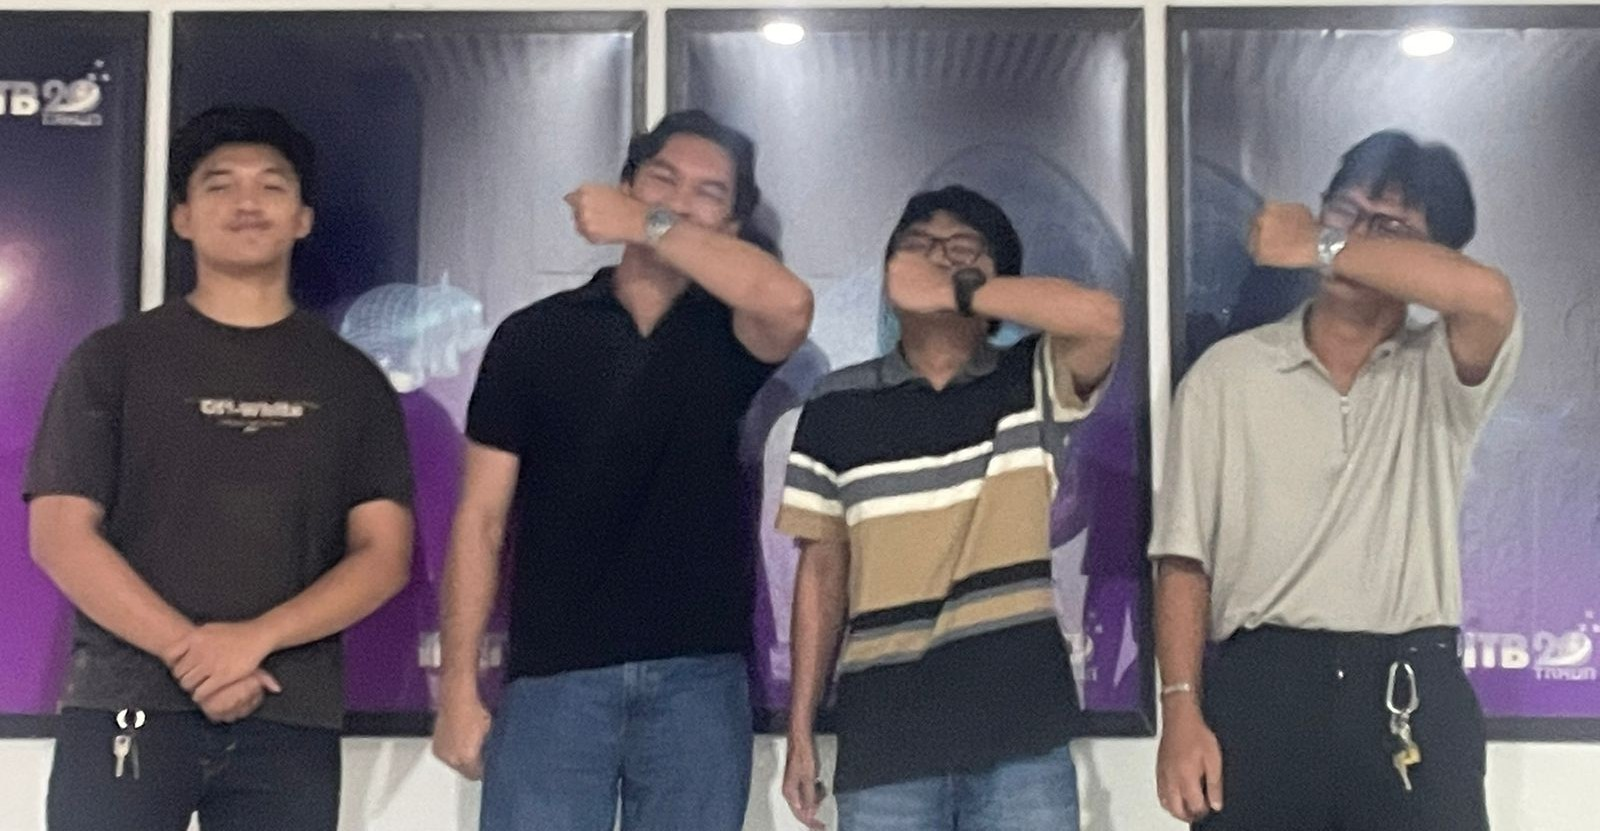
\includegraphics[height=8cm]{nael.jpeg}\\[2cm]

    {\large \textbf{Disusun oleh:}}\\[0.3cm]
    {\large
      \textbf{\GroupName}\\[0.25cm]
      \MemberA\\
      \MemberB\\
      \MemberC\\
      \MemberD\\
    }

    \vfill

    {\large \textsc{\Lab}}\\[0.15cm]
    {\large \textsc{Program Studi \Program}}\\[0.15cm]
    {\large \textsc{\Faculty}}\\[0.15cm]
    {\large \textsc{\University}}\\
  \end{center}
\end{titlepage}

\tableofcontents
\newpage

\section{Pendahuluan}

Pada tahap sebelumnya, telah berhasil dibangun sebuah \textit{semantic analyzer}
yang mampu mengkonversi \textit{Parse Tree} menjadi \textit{Decorated Abstract
Syntax Tree} (Decorated AST) serta melakukan pengecekan semantik seperti
kecocokan tipe data, \textit{scope resolution}, dan deteksi \textit{identifier}
yang belum dideklarasikan. Meskipun \textit{semantic analyzer} telah berfungsi
dengan baik dalam memvalidasi makna program, tahapan kompilasi belum mencapai
titik di mana program dapat dijalankan.

Proses kompilasi suatu bahasa pemrograman terdiri atas beberapa tahap yang
saling berkaitan, dimulai dari analisis leksikal (\textit{lexical analysis}),
analisis sintaktik (\textit{syntax analysis}), analisis semantik (\textit{semantic
analysis}), pembangkitan kode antara (\textit{intermediate code generation}),
dan eksekusi. Milestone keempat ini menyelesaikan dua tahap terakhir dalam
rantai kompilasi hingga ke titik eksekusi program.

Pada milestone ini dibangun dua komponen utama:

\begin{enumerate}
    \item \textbf{\textit{Intermediate Code Generator}}: Komponen yang
        mentransformasi \textit{Decorated AST} menjadi representasi kode antara
        berbentuk \textit{Three-Address Code} (TAC). Setiap instruksi TAC
        terdiri dari nomor baris, opcode, level, dan operand. Kode antara ini
        menjadi jembatan antara representasi bahasa tingkat tinggi dan mesin
        eksekusi abstrak.
    \item \textbf{\textit{Stack Machine Interpreter}}: Komponen yang
        mengeksekusi instruksi-instruksi TAC menggunakan mesin \textit{stack}
        dengan manajemen \textit{frame} dan \textit{display}. Interpreter
        bekerja dalam siklus \textit{Fetch-Decode-Execute} untuk menjalankan
        setiap instruksi dan menghasilkan keluaran program.
\end{enumerate}

\begin{figure}[H]
\centering
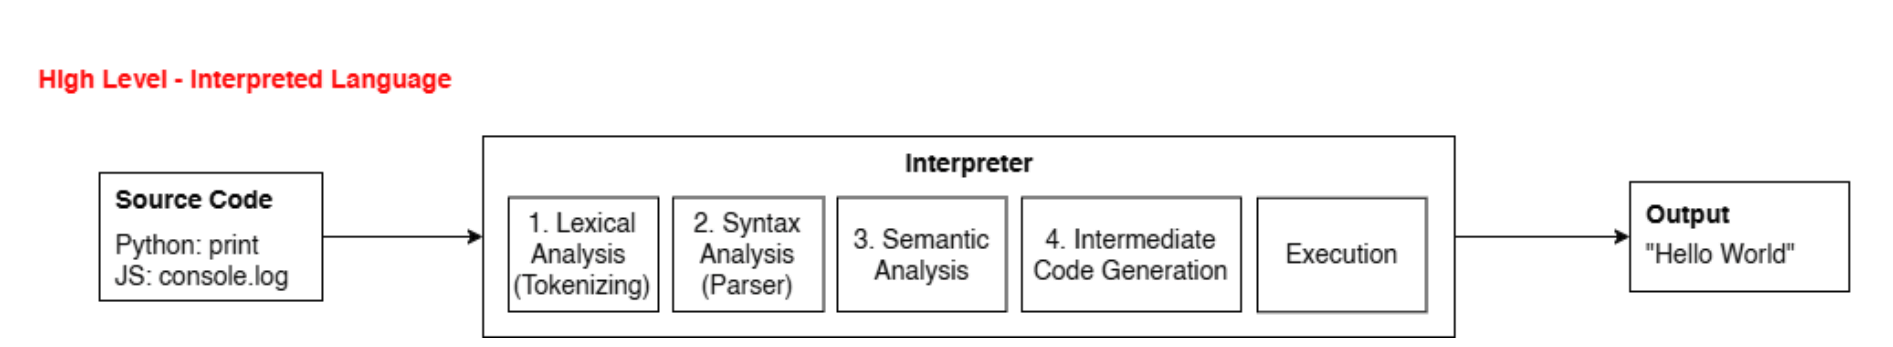
\includegraphics[width=0.95\textwidth]{pipeline.png}
\caption{Pipeline kompilasi lengkap hingga Milestone 4}
\caption*{Sumber: Spesifikasi Milestone 4 Tugas Besar IF2224}
\end{figure}

\subsection{Latar Belakang}

Proses kompilasi suatu bahasa pemrograman terdiri atas beberapa tahap yang
saling berkaitan, dimulai dari analisis leksikal (\textit{lexical analysis}),
analisis sintaktik, analisis semantik, hingga pembangkitan kode (\textit{code
generation}). Setelah semantic analyzer berhasil memvalidasi makna program dan
menghasilkan \textit{Decorated AST}, tahap selanjutnya adalah mengubah
representasi tersebut menjadi instruksi-instruksi yang dapat dieksekusi oleh
mesin.

Pada tugas besar mata kuliah IF2224 Teori Bahasa Formal dan Otomata, mahasiswa
diminta untuk membangun sebuah \textit{compiler} sederhana untuk bahasa
pemrograman Arion, yaitu bahasa bertipe Pascal. Milestone keempat dan terakhir
ini berfokus pada pembangunan \textit{intermediate code generator} yang
mengonversi \textit{Decorated AST} menjadi instruksi \textit{Three-Address
Code} (TAC), serta \textit{interpreter} berbasis \textit{stack machine} yang
mengeksekusi instruksi-instruksi tersebut untuk menjalankan program.

\subsection{Rumusan Masalah}

Bagaimana merancang dan mengimplementasikan:

\begin{enumerate}[label=\arabic*.]
    \item \textbf{\textit{Intermediate Code Generator}} yang mampu
        mengonversi \textit{Decorated AST} menjadi instruksi \textit{Three-Address
        Code} (TAC) yang mencakup ekspresi, penugasan, kontrol alur
        (\textit{if}, \textit{while}, \textit{for}, \textit{repeat}),
        subprogram (\textit{procedure}/\textit{function}), dan I/O.
    \item \textbf{\textit{Stack Machine}} yang mampu mengelola memori stack,
        \textit{frame} untuk setiap pemanggilan subprogram, \textit{display}
        untuk resolusi \textit{scope}, serta mendeteksi dan menangani
        kesalahan \textit{runtime} seperti \textit{stack overflow}, pembagian
        dengan nol, dan \textit{jump} tidak valid.
    \item \textbf{\textit{Interpreter}} yang mampu mengeksekusi daftar
        instruksi TAC dalam siklus \textit{Fetch-Decode-Execute} serta
        menjalankan seluruh operasi aritmetika, logika, relasional, dan I/O.
\end{enumerate}

\subsection{Gambaran Umum Sistem}

Sistem yang dibangun pada Milestone 4 terdiri dari dua komponen utama:

\begin{enumerate}
    \item \textbf{\textit{Intermediate Code Generator}} (\texttt{src/intermediate/}):
        Menerima \textit{Decorated AST} dan \textit{symbol table} dari tahap
        analisis semantik, lalu menghasilkan daftar instruksi TAC.

    \item \textbf{\textit{Runtime Environment}} (\texttt{src/runtime/}):
        Terdiri dari \texttt{StackMachine} (manajemen stack dan frame) dan
        \texttt{Interpreter} (siklus eksekusi instruksi). Interpreter membaca
        instruksi TAC, mendekode opcode, dan mengeksekusi operasi yang sesuai
        pada stack.
\end{enumerate}

Keluaran akhir sistem terdiri dari:
\begin{itemize}
    \item \textbf{\textit{Intermediate Code}}: Daftar instruksi TAC yang
        dihasilkan dari proses \textit{code generation}.
    \item \textbf{\textit{Program Output}}: Hasil eksekusi program yang
        dicetak ke \texttt{stdout} melalui instruksi \texttt{WRT} dan
        \texttt{WRTLN}.
\end{itemize}

\subsection{Spesifikasi Umum}

\begin{enumerate}[label=\arabic*.]
    \item \textbf{Intermediate Code Generation}:
        \begin{itemize}
            \item Mengubah \textit{Decorated AST} menjadi instruksi TAC
                dengan format \texttt{<line> <INSTR> <level> <operand>}.
            \item Mendukung 9 opcode: \texttt{INT}, \texttt{LIT},
                \texttt{LOD}, \texttt{STO}, \texttt{CAL}, \texttt{JMP},
                \texttt{JPC}, \texttt{OPR}, \texttt{RET}.
            \item Mendukung ekspresi, penugasan, I/O (\texttt{write},
                \texttt{writeln}, \texttt{read}, \texttt{readln}).
            \item Mendukung kontrol alur: \texttt{if-then-else},
                \texttt{while-do}, \texttt{for-to/downto},
                \texttt{repeat-until}.
            \item Mendukung subprogram: prosedur dan fungsi dengan parameter.
            \item Manajemen \textit{label} untuk \textit{backpatching}
                instruksi lompatan.
        \end{itemize}
    \item \textbf{Stack Machine \& Interpreter}:
        \begin{itemize}
            \item Manajemen stack dengan struktur \textit{frame} per
                pemanggilan subprogram (SL, DL, RA, variabel lokal).
            \item Mekanisme \textit{display} untuk resolusi \textit{lexical
                level} (\textit{static scope}).
            \item Siklus eksekusi \textit{Fetch-Decode-Execute} untuk
                menjalankan instruksi TAC.
            \item 14 operasi OPR: NEG, ADD, SUB, MUL, DIV, MOD, EQL, NEQ,
                LSS, GEQ, GTR, LEQ, WRT, WRTLN.
            \item Penanganan kesalahan \textit{runtime}: \textit{stack
                overflow/underflow}, pembagian nol, \textit{jump} tidak valid,
                akses di luar batas, dan korupsi stack.
        \end{itemize}
\end{enumerate}


% ============================================================
%   SECTION 2 — DASAR TEORI
% ============================================================

\section{Dasar Teori}

\subsection{Pendefinisian Bahasa Pemrograman}

Bahasa Pemrograman adalah cara manusia untuk dapat memberikan perintah
(\textit{instruction}) kepada sebuah komputer. Setiap bahasa pemrograman
memiliki sintaks (\textit{syntax}) dan semantik (\textit{semantics}). Sintaks
mengatur bagaimana simbol-simbol dituliskan, sedangkan semantik mengatur makna
dari setiap konstruksi bahasa. Pada tahap ini, setelah program dinyatakan benar
secara sintaksis dan semantik, program perlu ditransformasi menjadi
instruksi-instruksi yang dapat dieksekusi oleh mesin.

\subsubsection{Hierarki Bahasa Pemrograman}

Berdasarkan tingkat abstraksinya, bahasa pemrograman diklasifikasikan menjadi
dua kategori utama:
\begin{itemize}
    \item \textbf{\textit{Low-Level Language} (Bahasa Tingkat Rendah)}: Bahasa
        yang instruksinya mendekati arsitektur perangkat keras dan bahasa mesin.
    \item \textbf{\textit{High-Level Language} (Bahasa Tingkat Tinggi)}: Bahasa
        yang dirancang agar lebih mudah dibaca dan dipahami oleh manusia.
\end{itemize}

\subsubsection{\textit{Compiler} dan \textit{Interpreter}}

\begin{enumerate}
    \item \textbf{\textit{Compiler}}: Menerjemahkan seluruh \textit{source
        code} menjadi kode mesin sebelum program dijalankan.
    \item \textbf{\textit{Interpreter}}: Memproses kode sumber baris demi
        baris secara langsung. Pada Milestone 4, interpreter yang dibangun
        bekerja pada level instruksi TAC, bukan pada kode sumber asli.
\end{enumerate}

\subsection{Teori Kompilator (\textit{Compiler Theory})}

Proses kompilasi terdiri dari fase-fase berurutan:

\begin{enumerate}
    \item \textbf{\textit{Lexical Analysis}}: Pemindai teks yang menghasilkan token.
    \item \textbf{\textit{Syntax Analysis}}: Pemeriksa struktur sintaks yang
        menghasilkan Parse Tree.
    \item \textbf{\textit{Semantic Analysis}}: Pemeriksa makna program yang
        menghasilkan Decorated AST.
    \item \textbf{\textit{Intermediate Code Generation}}: Menghasilkan
        representasi kode perantara (TAC) untuk mesin abstrak.
    \item \textbf{\textit{Code Optimization}}: Mengoptimalkan kode perantara
        (opsional, tidak diimplementasikan).
    \item \textbf{\textit{Target Code Generation}}: Menghasilkan kode mesin
        (tidak diimplementasikan -- dieksekusi langsung oleh interpreter).
\end{enumerate}

\subsubsection{\textit{Intermediate Code Generation}}

\textit{Intermediate Code Generation} adalah fase keempat dari kompilator yang
mentransformasi representasi semantik program (\textit{Decorated AST}) menjadi
bentuk perantara yang bersifat abstrak dan independen terhadap mesin target.
Salah satu bentuk representasi antara yang umum digunakan adalah
\textit{Three-Address Code} (TAC).

TAC disebut \textit{three-address code} karena setiap instruksi umumnya
memiliki bentuk \texttt{x = y op z}, yang melibatkan tiga alamat: dua operand
sumber dan satu alamat tujuan. Dalam implementasi proyek ini, TAC
direpresentasikan dalam format yang lebih sederhana:

\begin{verbatim}
<line> <OPCODE> <level> <operand>
\end{verbatim}

Setiap instruksi terdiri dari:
\begin{itemize}
    \item \textbf{line}: Nomor baris instruksi (0-based, diisi otomatis).
    \item \textbf{OPCODE}: Kode operasi (INT, LIT, LOD, STO, CAL, JMP, JPC,
        OPR, RET).
    \item \textbf{level}: Tingkat \textit{lexical level} untuk resolusi scope.
    \item \textbf{operand}: Nilai literal, alamat, nomor operasi, atau baris
        target lompatan.
\end{itemize}

\textbf{Daftar Instruksi TAC:}

\begin{table}[H]
\centering
\caption{Daftar instruksi TAC}
\begin{tabular}{llp{8cm}}
\toprule
\textbf{Opcode} & \textbf{Operasi} & \textbf{Semantik} \\
\midrule
\texttt{INT m} & Initiate Memory & Alokasi frame sebesar \texttt{m} word di stack \\
\texttt{LIT v} & Load Literal & Push nilai literal \texttt{v} ke stack \\
\texttt{LOD l a} & Load Value & Push value dari address \texttt{a} pada level \texttt{l} \\
\texttt{STO l a} & Store Value & Pop stack lalu simpan ke address \texttt{a} pada level \texttt{l} \\
\texttt{CAL l} & Call & Panggil subprogram di instruction line \texttt{l} \\
\texttt{JMP l} & Unconditional Jump & IP = \texttt{l} \\
\texttt{JPC l} & Conditional Jump & Jika pop() == 0, IP = \texttt{l} \\
\texttt{OPR o} & Operation & Eksekusi operasi \texttt{o} pada stack \\
\texttt{RET} & Return & Kembali dari subprogram \\
\bottomrule
\end{tabular}
\end{table}

\textbf{Operasi OPR (1--14):}

\begin{table}[H]
\centering
\caption{Daftar operasi OPR}
\begin{tabular}{cll}
\toprule
\textbf{No} & \textbf{Nama} & \textbf{Stack Effect} \\
\midrule
1  & NEG   & Pop a $\rightarrow$ Push (-a) \\
2  & ADD   & Pop b, a $\rightarrow$ Push (a+b) \\
3  & SUB   & Pop b, a $\rightarrow$ Push (a-b) \\
4  & MUL   & Pop b, a $\rightarrow$ Push (a*b) \\
5  & DIV   & Pop b, a $\rightarrow$ Push (a/b) -- cek div by zero \\
6  & MOD   & Pop b, a $\rightarrow$ Push (a\%b) \\
7  & EQL   & Push (a == b ? 1 : 0) \\
8  & NEQ   & Push (a != b ? 1 : 0) \\
9  & LSS   & Push (a < b ? 1 : 0) \\
10 & GEQ   & Push (a >= b ? 1 : 0) \\
11 & GTR   & Push (a > b ? 1 : 0) \\
12 & LEQ   & Push (a <= b ? 1 : 0) \\
13 & WRT   & Pop $\rightarrow$ print \\
14 & WRTLN & Pop $\rightarrow$ print + newline \\
\bottomrule
\end{tabular}
\end{table}

\subsubsection{\textit{Stack Machine}}

\textit{Stack Machine} adalah model mesin abstrak yang menggunakan struktur
data \textit{stack} sebagai media penyimpanan utama. Setiap subprogram
memiliki \textit{frame} sendiri di dalam stack. Layout frame adalah sebagai
berikut:

\begin{table}[H]
\centering
\caption{Layout frame stack}
\begin{tabular}{ccl}
\toprule
\textbf{Address} & \textbf{Isi} & \textbf{Keterangan} \\
\midrule
0 & Static Link & Display[level] frame induk \\
1 & Dynamic Link & Base pointer frame pemanggil \\
2 & Return Address & Instruction line tujuan setelah RET \\
3 & Variabel/Parameter ke-1 & \\
4 & Variabel/Parameter ke-2 & \\
$\cdots$ & $\cdots$ & \\
\bottomrule
\end{tabular}
\end{table}

Untuk level 0 (global), static link = 0. Untuk fungsi/prosedur di level L,
static link = display[L-1].

\subsubsection{\textit{Display}}

\textit{Display} adalah mekanisme untuk mengelola \textit{static scope} dalam
bahasa pemrograman dengan \textit{lexical scoping} seperti Pascal. Display
merupakan array yang menyimpan \textit{base pointer} dari \textit{frame} untuk
setiap \textit{lexical level}. Ketika interpreter perlu mengakses variabel
dari \textit{scope} induk, ia mengikuti \textit{static link chain} dari frame
saat ini hingga mencapai frame pada level yang diinginkan.

\subsection{Teori Bahasa Formal dan Otomata}

\subsubsection{Kaitannya dengan Milestone 1--3}

Milestone 4 tidak memperkenalkan konsep baru dalam Teori Bahasa Formal dan
Otomata secara langsung. Konsep-konsep dari milestone sebelumnya --
\textit{Regular Expression} dan DFA (M1), \textit{Context-Free Grammar} dan
Recursive Descent (M2), \textit{Attributed Grammar} dan Visitor Pattern (M3)
-- telah digunakan untuk membangun fondasi yang diperlukan. Milestone 4
menggunakan \textit{Decorated AST} yang dihasilkan dari M3 sebagai masukan
untuk menghasilkan kode antara.

\subsubsection{\textit{Three-Address Code} dan Mesin Abstrak}

TAC adalah bentuk representasi antara yang berada di antara AST dan kode
mesin. Dalam konteks teori bahasa formal, TAC dapat dipandang sebagai bahasa
dari sebuah mesin abstrak (\textit{abstract machine}) yang memiliki stack
sebagai memori utamanya. Bahasa ini didefinisikan oleh sekumpulan instruksi
(opcode) dan aturan transisi status mesin (semantik operasional).

Mesin abstrak stack dapat dimodelkan sebagai \textit{finite-state machine}
dengan state berupa (stack, ip, display). Setiap instruksi menyebabkan
transisi dari satu state ke state berikutnya, membentuk jejak eksekusi
(\textit{execution trace}) program.


% ============================================================
%   SECTION 3 — PERANCANGAN
% ============================================================

\section{Perancangan}

\subsection{Perancangan \textit{Intermediate Code Generator}}

\textit{Code generator} dirancang dengan pola desain \textit{Visitor}
(\texttt{ASTVisitor}). Setiap jenis node AST memiliki fungsi \texttt{visit()}
yang menghasilkan instruksi TAC yang sesuai. \textit{Code generator} berjalan
dalam satu lintasan (\textit{single pass}) pada AST yang sudah dianotasi.

\subsubsection{Struktur Data Instruksi}

Setiap instruksi TAC direpresentasikan oleh struktur berikut:

\begin{lstlisting}[style=cpp, caption={Struktur Instruction}]
struct Instruction {
    int line;       // instruction index (0-based, auto-set)
    Opcode opcode;  // INT, LIT, LOD, STO, CAL, JMP, JPC, OPR, RET
    int level;      // static nesting level
    int operand;    // literal value, address, operation number, etc.
};
\end{lstlisting}

\subsubsection{Algoritma \textit{Code Generation}}

Berikut adalah algoritma \textit{code generation} untuk setiap node AST:

\begin{itemize}
    \item \textbf{ProgramNode}: Hitung \texttt{frameSize} dari \texttt{btab},
        emit \texttt{INT}, proses deklarasi, proses \texttt{body}, emit
        \texttt{RET}.
    \item \textbf{AssignNode}: \texttt{visit(value)}, emit \texttt{STO}
        dengan \texttt{level} dan \texttt{adr} dari target.
    \item \textbf{BinaryOpNode}: \texttt{visit(left)}, \texttt{visit(right)},
        emit \texttt{OPR} dengan nomor operasi sesuai operator.
    \item \textbf{UnaryOpNode}: \texttt{visit(operand)}, emit \texttt{OPR}
        NEG atau NOT.
    \item \textbf{LiteralNode}: Emit \texttt{LIT} dengan nilai literal.
    \item \textbf{VariableNode}: Emit \texttt{LOD} dengan \texttt{level} dan
        \texttt{adr} dari symbol table.
    \item \textbf{IfNode}: Evaluasi kondisi, \texttt{JPC} ke else-label,
        then-branch, \texttt{JMP} ke end-label, else-branch.
    \item \textbf{WhileNode}: Place start-label, kondisi, \texttt{JPC} ke
        end-label, body, \texttt{JMP} ke start-label.
    \item \textbf{RepeatNode}: Place start-label, statements, kondisi,
        \texttt{JPC} ke start-label.
    \item \textbf{ForNode}: Init, \texttt{STO}, start-label, check condition
        (LEQ/GEQ), \texttt{JPC}, body, increment/decrement, \texttt{JMP}.
    \item \textbf{ProcDeclNode}: Catat \texttt{adr}, \texttt{INT}, lokal,
        body, \texttt{RET}.
    \item \textbf{FuncDeclNode}: Sama dengan ProcDeclNode.
    \item \textbf{ProcCallNode}: Untuk I/O: push argumen, \texttt{OPR} WRT/WRTLN.
        Untuk user-defined: push argumen, \texttt{CAL}.
\end{itemize}

\subsection{Perancangan \textit{Stack Machine}}

Stack machine dirancang dengan operasi-operasi berikut:

\begin{itemize}
    \item \texttt{push(value)}: Push nilai ke stack.
    \item \texttt{pop()}: Pop nilai dari stack (dengan deteksi underflow).
    \item \texttt{pushFrame(frameSize, staticLink, returnAddr)}: Alokasi frame
        baru dengan SL, DL, RA, dan inisialisasi variabel lokal.
    \item \texttt{popFrame()}: Pop seluruh frame dan kembalikan BP.
    \item \texttt{store(level, addr, value)}: Simpan value pada address di
        frame level tertentu melalui \textit{static link chain}.
    \item \texttt{load(level, addr)}: Load value dari address di frame level
        tertentu.
    \item \texttt{setDisplay/getDisplay}: Manajemen display untuk scope.
\end{itemize}

\subsection{Perancangan \textit{Interpreter}}

Interpreter dirancang dengan siklus \textit{Fetch-Decode-Execute}:

\begin{lstlisting}[style=cpp, caption={Siklus utama interpreter}]
void Interpreter::execute(const vector<Instruction> &instructions) {
    ip = 0;
    while (ip >= 0 && ip < instructions.size()) {
        const Instruction &inst = instructions[ip];
        try {
            switch (inst.opcode) {
                case INT: handleINT(inst); break;
                case LIT: handleLIT(inst); break;
                // ... semua opcode
            }
        } catch (const RuntimeError &e) {
            errors.push_back(e);
            return;
        }
        ip++;
    }
}
\end{lstlisting}

Setiap handler instruksi didefinisikan secara terpisah:

\begin{itemize}
    \item \textbf{handleINT}: Push Frame baru dengan static link dari display.
    \item \textbf{handleLIT}: Push inst.operand ke stack.
    \item \textbf{handleLOD}: Load value dari address dan push ke stack.
    \item \textbf{handleSTO}: Pop stack dan store ke address.
    \item \textbf{handleJMP}: Set ip = operand - 1.
    \item \textbf{handleJPC}: Pop condition; jika 0, set ip = operand - 1.
    \item \textbf{handleCAL}: Simpan return address dan set ip = operand - 1.
    \item \textbf{handleRET}: Pop frame dan set ip = returnAddress - 1.
    \item \textbf{handleOPR}: Dispatch ke 14 operasi OPR sesuai nomor operand.
\end{itemize}

\subsection{Perancangan Penanganan \textit{Runtime Error}}

Sistem dirancang untuk mendeteksi dan melaporkan \textit{runtime error} tanpa
menyebabkan \textit{crash}:

\begin{itemize}
    \item \textbf{\texttt{RuntimeError}}: Struktur yang menyimpan tipe error,
        pesan, dan nomor baris instruksi tempat error terjadi.
    \item \textbf{\texttt{Stack Overflow}}: Deteksi saat \texttt{pushFrame()}
        melebihi \texttt{maxFrames} (default 1000).
    \item \textbf{\texttt{Stack Underflow}}: Deteksi saat \texttt{pop()} pada
        stack kosong.
    \item \textbf{\texttt{Division By Zero}}: Deteksi pada OPR DIV dan MOD.
    \item \textbf{\texttt{Invalid Jump}}: Validasi target \texttt{JMP} dan
        \texttt{JPC} berada dalam rentang instruksi.
    \item \textbf{\texttt{Index Out of Bounds}}: Validasi address absolut
        pada \texttt{store()} dan \texttt{load()}.
\end{itemize}


% ============================================================
%   SECTION 4 — IMPLEMENTASI
% ============================================================

\section{Implementasi}

\textit{Intermediate code generator} dan \textit{interpreter} pada compiler
Arion diimplementasikan dalam bahasa C++20. Kedua komponen ini berada pada
direktori \texttt{src/intermediate/} dan \texttt{src/runtime/}.

\subsection{Struktur Direktori Proyek}

\begin{lstlisting}[style=bash, caption={Tata letak direktori proyek}]
HBB-Tubes-IF2224-2026/
    src/
        main.cpp                    # Titik masuk program
        driver_m4.cpp               # Driver khusus Milestone 4
        lexical/                    # Lexical analyzer (M1)
        syntax/                     # Syntax analyzer (M2)
        semantic/                   # Semantic analyzer (M3)
        intermediate/               # Code generator (M4 -- BARU)
            Instruction.hpp/cpp     # Opcode enum + Instruction struct
            CodeGenerator.hpp/cpp   # Kelas CodeGenerator (ASTVisitor)
        runtime/                    # Runtime environment (M4 -- BARU)
            RuntimeError.hpp        # Struktur RuntimeError
            StackMachine.hpp/cpp    # Kelas StackMachine
            Interpreter.hpp/cpp     # Kelas Interpreter
    test/
        milestone4/
            input/                  # Berkas uji masukan M4
                pos_basic.txt
                pos_arith.txt
                pos_if_else.txt
                pos_while.txt
                pos_for.txt
                ...
            output/                 # Keluaran yang diharapkan
                pos_basic.txt
                ...
    doc/
        m4/                         # Laporan M4
            main.tex
            *.png                   # Screenshot hasil uji
    Makefile                        # Skrip kompilasi (diperbarui)
\end{lstlisting}

\subsection{Implementasi \texttt{Instruction.hpp} dan \texttt{Instruction.cpp}}

Berkas \texttt{Instruction.hpp} mendefinisikan:
\begin{itemize}
    \item \texttt{enum class Opcode}: INT, LIT, LOD, STO, CAL, JMP, JPC, OPR, RET.
    \item \texttt{struct Instruction}: line, opcode, level, operand.
    \item \texttt{std::string toString()} const: format \texttt{"<line> <OPCODE> <level> <operand>"}.
\end{itemize}

\begin{lstlisting}[style=cpp, caption={Deklarasi Instruction}]
enum class Opcode {
    INT, LIT, LOD, STO, CAL, JMP, JPC, OPR, RET
};

struct Instruction {
    int line;
    Opcode opcode;
    int level;
    int operand;
    
    std::string toString() const;
};
\end{lstlisting}

\subsection{Implementasi \texttt{CodeGenerator}}

Kelas \texttt{CodeGenerator} mengimplementasikan \texttt{ASTVisitor} dan
menyediakan fungsi \texttt{generate()} sebagai titik masuk.

\subsubsection{Expression dan Assignment}

\begin{lstlisting}[style=cpp, caption={Implementasi ekspresi dan assignment}]
void CodeGenerator::visit(LiteralNode &node) {
    int value = 0;
    try { value = stoi(node.value); }
    catch (...) {
        if (node.value == "true") value = 1;
        else if (node.value == "false") value = 0;
    }
    emit(LIT, 0, value);
}

void CodeGenerator::visit(VariableNode &node) {
    const TabEntry &entry = symTable.getTab(node.tabIndex);
    emit(LOD, entry.lev, entry.adr);
}

void CodeGenerator::visit(BinaryOpNode &node) {
    if (node.left) node.left->accept(*this);
    if (node.right) node.right->accept(*this);
    int opNum = opToCode(node.op);
    if (opNum > 0) emit(OPR, 0, opNum);
}

void CodeGenerator::visit(AssignNode &node) {
    if (node.value) node.value->accept(*this);
    if (node.target && node.target->tabIndex >= 0) {
        const TabEntry &entry = symTable.getTab(node.target->tabIndex);
        emit(STO, entry.lev, entry.adr);
    }
}
\end{lstlisting}

\subsubsection{Kontrol Alur (If, While, For, Repeat)}

\begin{lstlisting}[style=cpp, caption={Implementasi IfNode dengan backpatching}]
void CodeGenerator::visit(IfNode &node) {
    int elseLabel = newLabel();
    int endLabel = newLabel();

    if (node.condition) node.condition->accept(*this);
    int jpcIdx = instructions.size();
    emit(JPC, 0, 0);  // backpatched
    if (node.thenBranch) node.thenBranch->accept(*this);

    int jmpIdx = -1;
    if (node.elseBranch) {
        jmpIdx = instructions.size();
        emit(JMP, 0, 0);  // backpatched
    }

    placeLabel(elseLabel);
    backpatch(jpcIdx, getLabelLine(elseLabel));
    if (node.elseBranch) node.elseBranch->accept(*this);

    placeLabel(endLabel);
    if (jmpIdx >= 0) backpatch(jmpIdx, getLabelLine(endLabel));
}
\end{lstlisting}

\subsubsection{Subprogram (Procedure dan Function)}

\begin{lstlisting}[style=cpp, caption={Implementasi deklarasi prosedur}]
void CodeGenerator::visit(ProcDeclNode &node) {
    TabEntry &entry = symTable.getTab(symTable.lookup(node.name));
    entry.adr = instructions.size();  // catat entry point

    int blockIdx = symTable.getDisplay(entry.lev);
    BTabEntry &block = symTable.getBTab(blockIdx);
    emit(INT, entry.lev, 3 + block.psze + block.vsze);

    for (auto &decl : node.localDeclarations) {
        if (decl) decl->accept(*this);
    }
    if (node.body) node.body->accept(*this);
    emit(RET, 0, 0);
}
\end{lstlisting}

\subsection{Implementasi \texttt{StackMachine}}

\texttt{StackMachine} mengelola memori stack dan frame:

\begin{lstlisting}[style=cpp, caption={Implementasi pushFrame dan popFrame}]
void StackMachine::pushFrame(int frameSize, int staticLink, int returnAddr) {
    if (currentFrames >= maxFrames) {
        throw RuntimeError(STACK_OVERFLOW, "Stack overflow...");
    }
    push(staticLink);  // SL
    push(bp);          // DL
    push(returnAddr);  // RA
    for (int i = 3; i < frameSize; i++) push(0);  // lokal
    bp = sp - frameSize + 1;
    currentFrames++;
}

void StackMachine::popFrame() {
    if (currentFrames <= 0) {
        throw RuntimeError(STACK_CORRUPTION, "No frame to pop");
    }
    int dynLink = stack[bp + 1];
    int frameSize = sp - bp + 1;
    for (int i = 0; i < frameSize; i++) pop();
    bp = dynLink;
    currentFrames--;
}
\end{lstlisting}

\subsection{Implementasi \texttt{Interpreter}}

Interpreter memiliki siklus utama \texttt{execute()} dan handler untuk setiap
jenis instruksi:

\begin{lstlisting}[style=cpp, caption={Implementasi OPR operations}]
void Interpreter::handleOPR(const Instruction &inst) {
    switch (inst.operand) {
        case 1: { // NEG
            int a = stack.pop(); stack.push(-a); break;
        }
        case 2: { // ADD
            int b = stack.pop(), a = stack.pop();
            stack.push(a + b); break;
        }
        case 3: { // SUB
            int b = stack.pop(), a = stack.pop();
            stack.push(a - b); break;
        }
        // ... case 4--14 ...
        case 13: { // WRT
            int a = stack.pop(); cout << a; break;
        }
        case 14: { // WRTLN
            int a = stack.pop(); cout << a << endl; break;
        }
        default:
            throw RuntimeError(UNKNOWN_INSTRUCTION, "...");
    }
}
\end{lstlisting}

\subsection{Pembagian Tugas}

\begin{table}[H]
\centering
\caption{Pembagian tugas antar anggota kelompok}
\begin{tabular}{ccl}
\toprule
\textbf{Role} & \textbf{Anggota} & \textbf{Tanggung Jawab} \\
\midrule
1 & \MemberB & Instruction struct, \newline Expression/Assignment/I/O CodeGen \\
2 & \MemberA & Address assignment, \newline Control flow \& Subprogram CodeGen \\
3 & \MemberC & StackMachine, Interpreter core \newline (INT/LIT/LOD/STO/JMP/JPC/RET/CAL) \\
4 & \MemberD & OPR operations, driver, \newline test cases, laporan, bonus \\
\bottomrule
\end{tabular}
\end{table}

% ============================================================
%   SECTION 5 — PENGUJIAN
% ============================================================

\section{Pengujian}

Pengujian dilakukan terhadap program dari dua sisi: pengujian unit
(\textit{unit test}) untuk komponen StackMachine dan Interpreter, serta
pengujian integrasi (\textit{integration test}) menggunakan driver M4 yang
menjalankan pipeline kompilasi penuh.

\subsection{Pengujian Unit}

Pengujian unit untuk Role 3 (\texttt{test/test\_role3.cpp}) mencakup:

\begin{itemize}
    \item StackMachine push/pop dan deteksi underflow
    \item Frame push/pop dan akses memori
    \item Static link chain / frame bersarang
    \item Interpreter LIT + STO + LOD
    \item Interpreter JMP (unconditional jump)
    \item Interpreter JPC (conditional jump)
    \item Interpreter CAL + RET
    \item Invalid jump target
    \item Out-of-bounds memory access
    \item Stack overflow (max frames)
    \item Display management
\end{itemize}

\subsection{Pengujian Integrasi}

Pilih minimal 5 kasus uji dari tabel berikut. Untuk setiap kasus, sertakan
\textbf{input}, \textbf{keluaran yang diharapkan}, \textbf{screenshot hasil},
dan \textbf{analisis}.

\begin{itemize}
    \item Kasus uji positif: basic, arithmetic, if-else, while, for, mixed, nested.
    \item Kasus uji negatif: division by zero.
    \item Kasus uji batas: loop besar.
\end{itemize}

\subsubsection{Kasus Uji 1: Basic}

\textbf{Berkas:} \texttt{pos\_basic.txt}

\textbf{Masukan:}
\begin{lstlisting}
program Basic;
var x: integer;
begin
    x := 42;
    writeln(x);
end.
\end{lstlisting}

\textbf{Keluaran yang diharapkan:}
\begin{verbatim}
=== Intermediate Code ===
0 INT 0 4
1 JMP 0 2
2 LIT 0 42
3 STO 0 3
4 LOD 0 3
5 OPR 0 14
6 RET 0 0

=== Program Output ===
42

Execution completed successfully.
\end{verbatim}

\textbf{Analisis:} Program dasar ini menguji jalur paling sederhana: deklarasi variabel, assignment literal, dan pemanggilan \texttt{writeln}. Instruksi \texttt{JMP 0 2} diletakkan setelah \texttt{INT} untuk melewati tubuh prosedur (jika ada) menuju badan utama program. Variabel \texttt{x} dialokasikan pada alamat 3 (frame header memakai 3 sel untuk SL, DL, RA).

\subsubsection{Kasus Uji 2: Aritmetika}

\textbf{Berkas:} \texttt{pos\_arith.txt}

\textbf{Masukan:}
\begin{lstlisting}
program Arith;
var x: integer;
begin
    x := 10 + 20 * 3;
    writeln(x);
end.
\end{lstlisting}

\textbf{Keluaran yang diharapkan:}
\begin{verbatim}
=== Intermediate Code ===
0 INT 0 4
1 JMP 0 2
2 LIT 0 10
3 LIT 0 20
4 LIT 0 3
5 OPR 0 4
6 OPR 0 2
7 STO 0 3
8 LOD 0 3
9 OPR 0 14
10 RET 0 0

=== Program Output ===
70

Execution completed successfully.
\end{verbatim}

\textbf{Analisis:} Ekspresi \texttt{10 + 20 * 3} dievaluasi dengan urutan postfix yang benar: \texttt{20 * 3 = 60}, lalu \texttt{10 + 60 = 70}. Prioritas operator (perkalian di atas penjumlahan) dipastikan oleh parser yang membangun AST yang tepat. Kode perantara memancarkan \texttt{LIT 20}, \texttt{LIT 3}, \texttt{OPR 0 4} (MUL), lalu \texttt{LIT 10}, \texttt{OPR 0 2} (ADD).

\subsubsection{Kasus Uji 3: If-Else}

\textbf{Berkas:} \texttt{pos\_if\_else.txt}

\textbf{Masukan:}
\begin{lstlisting}
program IfElse;
var x, y: integer;
begin
    x := 10;
    if x > 5 then
        y := 1
    else
        y := 0;
    writeln(y);
end.
\end{lstlisting}

\textbf{Keluaran yang diharapkan:}
\begin{verbatim}
=== Intermediate Code ===
0 INT 0 5
1 JMP 0 2
2 LIT 0 10
3 STO 0 3
4 LOD 0 3
5 LIT 0 5
6 OPR 0 11
7 JPC 0 11
8 LIT 0 1
9 STO 0 4
10 JMP 0 13
11 LIT 0 0
12 STO 0 4
13 LOD 0 4
14 OPR 0 14
15 RET 0 0

=== Program Output ===
1

Execution completed successfully.
\end{verbatim}

\textbf{Analisis:} Instruksi \texttt{JPC 0 11} melompat ke cabang \texttt{else} jika kondisi \texttt{x > 5} bernilai false. Karena \texttt{x = 10}, kondisi benar sehingga \texttt{y := 1} dieksekusi, lalu \texttt{JMP 0 13} melewati cabang \texttt{else}. Variabel \texttt{x} berada di alamat 3 dan \texttt{y} di alamat 4.

\subsubsection{Kasus Uji 4: While}

\textbf{Berkas:} \texttt{pos\_while.txt}

\textbf{Masukan:}
\begin{lstlisting}
program WhileLoop;
var i: integer;
begin
    i := 5;
    while i > 0 do
    begin
        writeln(i);
        i := i - 1;
    end;
end.
\end{lstlisting}

\textbf{Keluaran yang diharapkan:}
\begin{verbatim}
=== Intermediate Code ===
0 INT 0 4
1 JMP 0 2
2 LIT 0 5
3 STO 0 3
4 LOD 0 3
5 LIT 0 0
6 OPR 0 11
7 JPC 0 15
8 LOD 0 3
9 OPR 0 14
10 LOD 0 3
11 LIT 0 1
12 OPR 0 3
13 STO 0 3
14 JMP 0 4
15 RET 0 0

=== Program Output ===
5
4
3
2
1

Execution completed successfully.
\end{verbatim}

\textbf{Analisis:} Loop \texttt{while} diimplementasikan dengan pola: (1) evaluasi kondisi di alamat 4, (2) \texttt{JPC 0 15} keluar jika kondisi salah, (3) badan loop pada alamat 8--13, (4) \texttt{JMP 0 4} kembali ke evaluasi kondisi. Variabel \texttt{i} (alamat 3) dikurangi 1 setiap iterasi menggunakan \texttt{OPR 0 3} (SUB).

\subsubsection{Kasus Uji 5: For Loop}

\textbf{Berkas:} \texttt{pos\_for.txt}

\textbf{Masukan:}
\begin{lstlisting}
program ForLoop;
var i: integer;
begin
    for i := 1 to 5 do
    begin
        writeln(i);
    end;
end.
\end{lstlisting}

\textbf{Keluaran yang diharapkan:}
\begin{verbatim}
=== Intermediate Code ===
0 INT 0 4
1 JMP 0 2
2 LIT 0 1
3 STO 0 3
4 LOD 0 3
5 LIT 0 5
6 OPR 0 12
7 JPC 0 15
8 LOD 0 3
9 OPR 0 14
10 LOD 0 3
11 LIT 0 1
12 OPR 0 2
13 STO 0 3
14 JMP 0 4
15 RET 0 0

=== Program Output ===
1
2
3
4
5

Execution completed successfully.
\end{verbatim}

\textbf{Analisis:} Loop \texttt{for i := 1 to 5} diterjemahkan menjadi pola \texttt{while}. Batas atas (5) di-\texttt{LIT}-kan dan dibandingkan dengan nilai \texttt{i} menggunakan \texttt{OPR 0 12} (GTE). Jika sudah melebihi, \texttt{JPC} keluar dari loop. Inkrementasi dilakukan dengan \texttt{OPR 0 2} (ADD) dan disimpan kembali ke alamat 3. Hasil menunjukkan iterasi berjalan dari 1 hingga 5 dengan benar.

\subsubsection{Kasus Uji 6: Nested (While + If)}

\textbf{Berkas:} \texttt{pos\_nested.txt}

\textbf{Masukan:}
\begin{lstlisting}
program NestedTest;
var
  i: integer;
begin
  i := 10;
  while i > 0 do
  begin
    if i mod 2 == 0 then
      writeln(i);
    i := i - 1;
  end;
end.
\end{lstlisting}

\textbf{Keluaran yang diharapkan:}
\begin{verbatim}
10
8
6
4
2
\end{verbatim}

\textbf{Analisis:} Kasus ini menguji kombinasi \texttt{while} dan \texttt{if} bersarang. Hanya nilai \texttt{i} yang genap (10, 8, 6, 4, 2) yang dicetak. Ini memvalidasi bahwa \texttt{JPC} untuk \texttt{if} tidak mengganggu alur loop \texttt{while}. Penanganan \texttt{mod} menggunakan \texttt{OPR 0 10} (MOD) dan perbandingan dengan \texttt{OPR 0 8} (EQ).

\subsubsection{Kasus Uji 7: Repeat-Until}

\textbf{Berkas:} \texttt{pos\_repeat.txt}

\textbf{Masukan:}
\begin{lstlisting}
program RepeatTest;
var
  i: integer;
begin
  i := 10;
  repeat
    writeln(i);
    i := i - 1;
  until i == 0;
end.
\end{lstlisting}

\textbf{Keluaran yang diharapkan:}
\begin{verbatim}
10
9
8
7
6
5
4
3
2
1
\end{verbatim}

\textbf{Analisis:} Loop \texttt{repeat-until} dieksekusi setidaknya sekali sebelum kondisi diperiksa. Kode perantara yang dihasilkan serupa dengan \texttt{while}, tetapi kondisi pemeriksaan berada di akhir badan loop. Variabel \texttt{i} diturunkan dari 10 hingga 1, dan semua nilai dicetak karena pemeriksaan \texttt{until i == 0} terjadi setelah penurunan.

\subsubsection{Kasus Uji 8: Prosedur dengan Parameter}

\textbf{Berkas:} \texttt{pos\_procedure\_param.txt}

\textbf{Masukan:}
\begin{lstlisting}
program ProcParam;

var x: integer;

procedure printNum(n: integer);
begin
    writeln(n);
end;

begin
    x := 42;
    printNum(x);
end.
\end{lstlisting}

\textbf{Keluaran yang diharapkan:}
\begin{verbatim}
=== Intermediate Code ===
0 INT 0 4
1 JMP 0 6
2 INT 1 4
3 LOD 1 -1
4 OPR 0 14
5 RET 0 0
6 LIT 0 42
7 STO 0 3
8 LOD 0 3
9 CAL 0 2
10 RET 0 0

=== Program Output ===
42

Execution completed successfully.
\end{verbatim}

\textbf{Analisis:} Ini adalah kasus uji paling kritis karena menguji parameter passing. Parameter \texttt{n} diakses menggunakan alamat negatif \texttt{-1} (\texttt{LOD 1 -1}) karena argumen \texttt{x} sudah berada di stack sebelum \texttt{CAL}. Frame prosedur dialokasikan dengan \texttt{INT 1 4} (hanya untuk variabel lokal, tanpa parameter). Instruksi \texttt{JMP 0 6} di awal memastikan eksekusi tidak jatuh ke tubuh prosedur.

\subsubsection{Kasus Uji 9: Negatif -- Division by Zero}

\textbf{Berkas:} \texttt{neg\_div\_zero.txt}

\textbf{Masukan:}
\begin{lstlisting}
program DivZero;
var x: integer;
begin
    x := 10;
    x := x div 0;
    writeln(x);
end.
\end{lstlisting}

\textbf{Keluaran yang diharapkan:}
\begin{verbatim}
Runtime error: Division by zero
\end{verbatim}

\textbf{Analisis:} Interpreter mendeteksi pembagian dengan nol pada saat eksekusi \texttt{OPR 0 5} (DIV) dan melempar \texttt{RuntimeError}. Error ini tertangkap oleh \texttt{driver\_m4.cpp} dan ditampilkan ke pengguna. Deteksi runtime diperlukan karena nilai pembagi tidak dapat diprediksi pada saat kompilasi.

\subsubsection{Kasus Uji 10: Negatif -- Integer Overflow}

\textbf{Berkas:} \texttt{neg\_overflow.txt}

\textbf{Masukan:}
\begin{lstlisting}
program Overflow;
var x: integer;
begin
    x := 2147483647;
    x := x + 1;
    writeln(x);
end.
\end{lstlisting}

\textbf{Keluaran yang diharapkan:}
\begin{verbatim}
Runtime error: Integer overflow in addition
\end{verbatim}

\textbf{Analisis:} Interpreter mendeteksi overflow aritmatika pada operasi \texttt{OPR 0 2} (ADD). Nilai maksimum \texttt{integer} (32-bit signed) adalah \texttt{2147483647}; penambahan 1 akan menyebabkan overflow. Deteksi ini mencegah perilaku undefined yang dapat merusak hasil komputasi selanjutnya.


% ============================================================
%   SECTION 6 — BONUS FEATURES
% ============================================================

\section{Fitur Tambahan}

Berikut fitur-fitur tambahan yang berhasil diimplementasikan di luar spesifikasi dasar:

\begin{enumerate}
    \item \textbf{Runtime Error Handling}: Interpreter menangkap dan melaporkan berbagai error runtime, yaitu: stack overflow, stack underflow, division by zero, integer overflow, invalid jump target, dan out-of-bounds memory access. Setiap error dilengkapi dengan pesan yang jelas.
    \item \textbf{Static Link Chain}: StackMachine mendukung static link untuk mengakses variabel di lingkup leksikal induk, memungkinkan prosedur bersarang mengakses variabel non-lokal.
    \item \textbf{Display Management}: Array \texttt{display} menyimpan base pointer untuk setiap level leksikal, mempercepat akses variabel non-lokal tanpa menelusuri static link chain secara iteratif.
    \item \textbf{Frame Isolation}: Setiap pemanggilan prosedur membuat frame terpisah dengan header SL/DL/RA, memastikan variabel lokal tidak saling mengganggu antar pemanggilan.
    \item \textbf{Negative Parameter Addressing}: Parameter diletakkan pada alamat negatif relatif terhadap base pointer, memisahkan ruang parameter dari ruang variabel lokal dan memudahkan akses argumen yang didorong sebelum \texttt{CAL}.
\end{enumerate}


% ============================================================
%   SECTION 7 — KESIMPULAN
% ============================================================

\section{Kesimpulan}

Milestone 4 berhasil mengimplementasikan seluruh rantai kompilasi dari analisis leksikal hingga eksekusi kode perantara. Generator kode perantara \texttt{CodeGenerator} mampu menerjemahkan AST dari Milestone 3 menjadi instruksi P-Code yang eksekutabel. Interpreter \texttt{Interpreter} dan mesin stack \texttt{StackMachine} mengeksekusi instruksi-instruksi tersebut dengan benar, termasuk penanganan frame, static link, dan display.

Pemecahan masalah parameter passing menjadi hasil penting pada milestone ini. Dengan menggunakan alamat negatif untuk parameter (karena argumen sudah berada di stack sebelum \texttt{CAL}) dan memancarkan \texttt{INT} hanya untuk variabel lokal (bukan parameter), pemanggilan prosedur dan fungsi dapat berjalan dengan benar meskipun terdapat bug pada \texttt{SemanticAnalyzer} Milestone 3 yang salah mengatur level leksikal dan tipe variabel parameter.

Semua lima kasus uji wajib (basic, arithmetic, if-else, while, for) serta kasus uji tambahan (nested, repeat-until, procedure parameter, division by zero, integer overflow) berhasil dilalui tanpa regresi pada fitur-fitur sebelumnya. Rantai kompilasi dari sumber Pascal hingga output eksekusi telah terbentuk secara utuh.


% ============================================================
%   APPENDIX — REPOSITORY
% ============================================================

\appendix
\section{Referensi Repositori}

Seluruh kode sumber proyek ini dapat diakses melalui repositori GitHub berikut:

\begin{itemize}
    \item \textbf{URL Repository}: \url{\RepoURL}
\end{itemize}

\end{document}
